\documentclass[
size=17pt,
paper=smartboard,
mode=present,
display=slidesnotes,
style=paintings,
nopagebreaks,
blackslide,
fleqn]{powerdot}

% styles: sailor, paintings
% wj capsules prettybox
% mode = handout or present


\usepackage{amsmath,graphicx,color,amsfonts}
\usepackage[brazilian]{babel}
\usepackage[utf8]{inputenc}
\newcommand{\palette}{Europa}


% palettes:
%    - sailor: Sea, River, Wine, Chocolate, Cocktail 
%    - paintings: Syndics, Skater, GoldenGate, Moitessier, PearlEarring, Lamentation, HolyWood, Europa, MayThird, Charon 

\newcommand{\cursopequeno}{EC01008 AOC}
\newcommand{\cursogrande}{\Large EC01008 -- Arquitetura e organização de computadores}



\author{Ronaldo de Freitas Zampolo\\FCT-ITEC-UFPA}
\date{2023-4}


\pdsetup{
   lf = {\cursopequeno},
   rf = {Componentes e função}, palette = {\palette}, randomdots={false},
   cf = {\theslide}
}


%opening
\title{\cursogrande\\ \vspace{1cm}Componentes e função de um computador}

\begin{document}
   \maketitle[randomdots={false}]
   
   \begin{slide}{Agenda}
      \tableofcontents[content=sections]
   \end{slide}
%%%%%%%%%%%%%%%%%%%%%%%%%%%%%%%%%%%%%%%%%%%%%%%%%%%%%%
\section[slide=true]{Componentes do computador}
\begin{slide}{Conceitos principais}
	Princípios da máquina de Von Neumann:
   \begin{itemize}
     \item Dados e instruções: armazenados em uma única memória
     \item Conteúdo da memória: 
	     \begin{itemize}
		     \item Endereçável por local (posição de memória)
		     \item Tipo de dado não considerado
	     \end{itemize}
     \item Padrão sequencial de execução
   \end{itemize}
\end{slide}

\begin{slide}{Software \emph{versus} Hardware}
   \centering
   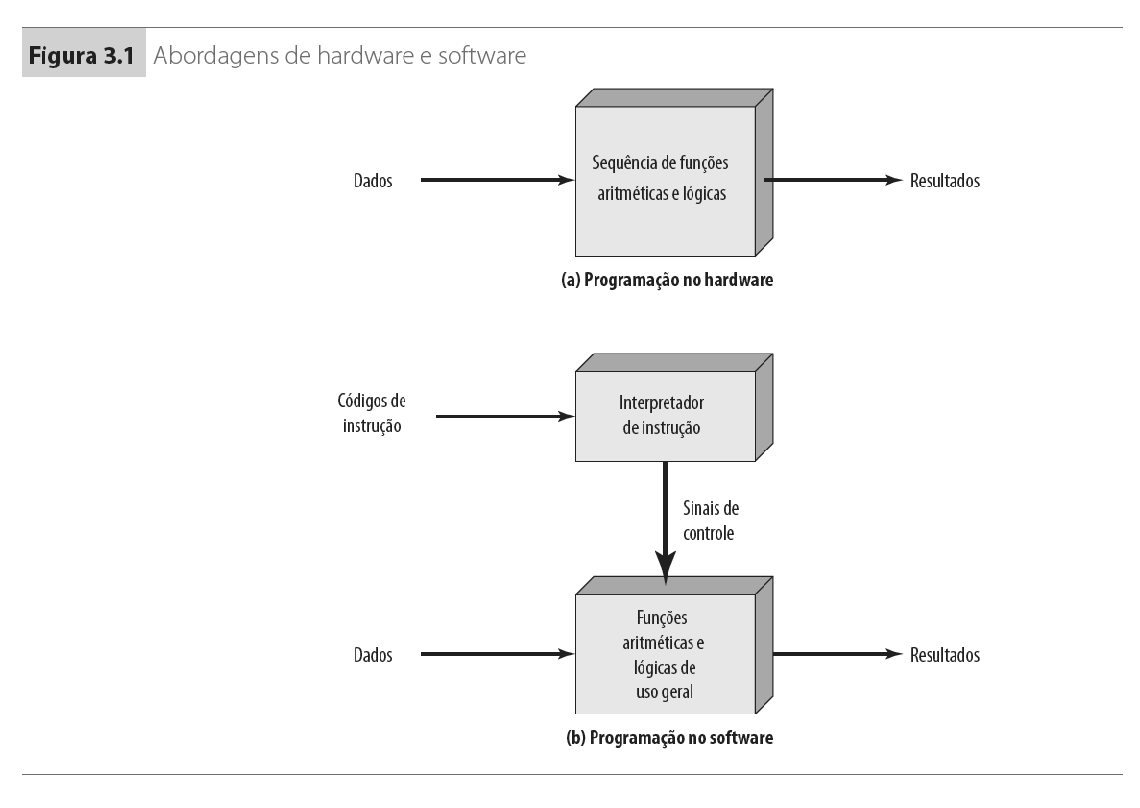
\includegraphics[scale=0.95]{figs/softhard.eps}
\end{slide}

\begin{slide}{Visão de alto nível}
   \centering
   \includegraphics[scale=0.95]{figs/altonivel.eps}
\end{slide}

\section[slide=true]{Função do computador}
\begin{slide}{Busca e execução de instruções}
\begin{itemize}
   \item Função básica: execução de um programa
   \item Programa: conjunto de instruções armazenadas na memória
   \item Ciclo de instrução:
   \begin{itemize}
      \item Ciclo de busca: leitura de instruções, uma de cada vez
      \item Ciclo de execução: cada instrução é interpretada e executada\pause
   \end{itemize}
   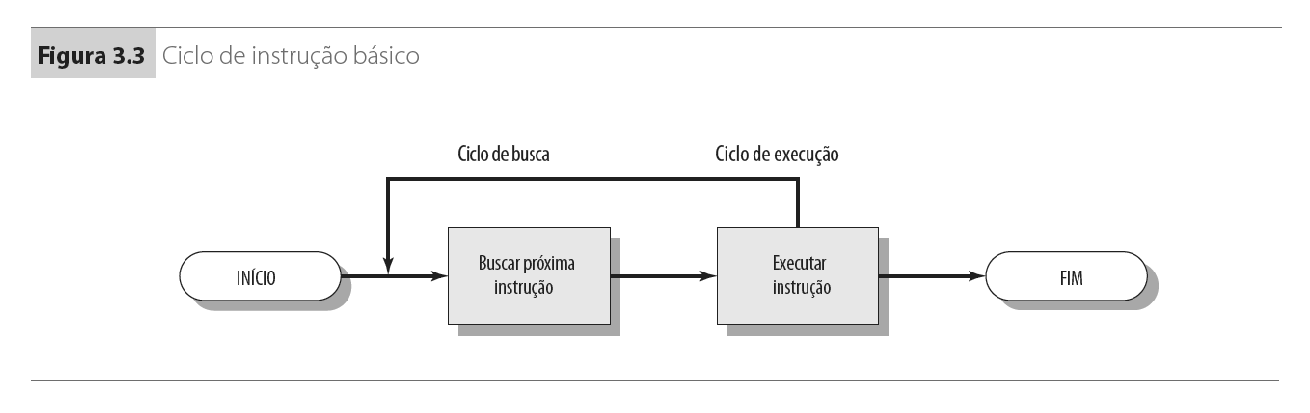
\includegraphics[width=\textwidth]{figs/cicloinstrucao.eps}
\end{itemize}
\end{slide}

\begin{slide}{Ciclo de instrução}
\begin{itemize}
   \item PC
   \begin{itemize}
      \item Registrador que armazena endereço da instrução
      \item Valor armazenado é incrementado após cada busca de instrução (salvo se houver algum desvio)
   \end{itemize}
   \item IR: registrador que armazena a instrução lida
   \item Tipos de ações:
   \begin{itemize}
      \item Processador-memória
      \item Processador-E/S
      \item Processamento de dados
      \item Controle
   \end{itemize}
\end{itemize}
\end{slide}

\begin{slide}{Máquina hipotética}
   \centering
   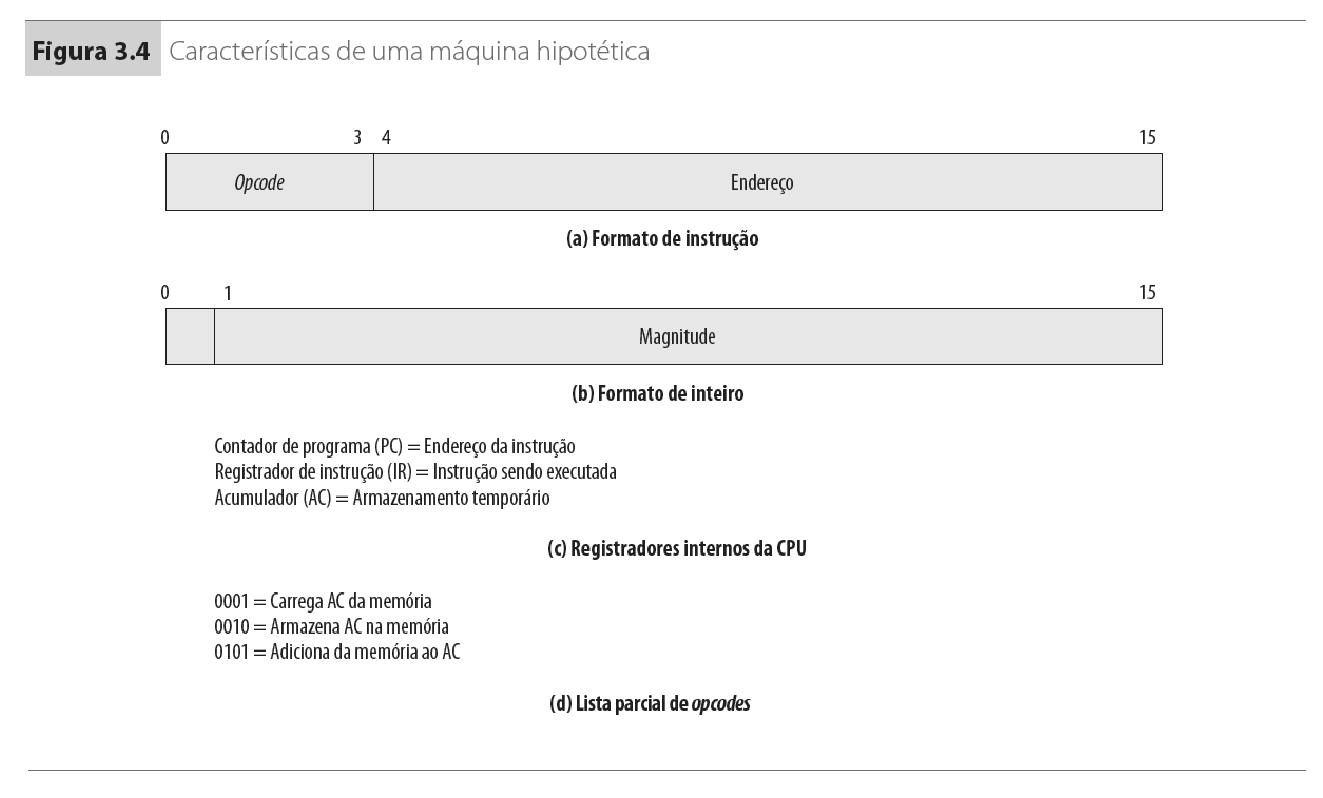
\includegraphics[width=0.9\textwidth]{figs/maquinahpt.eps}
\end{slide}

\begin{slide}{Exemplo de execução}
   \centering
   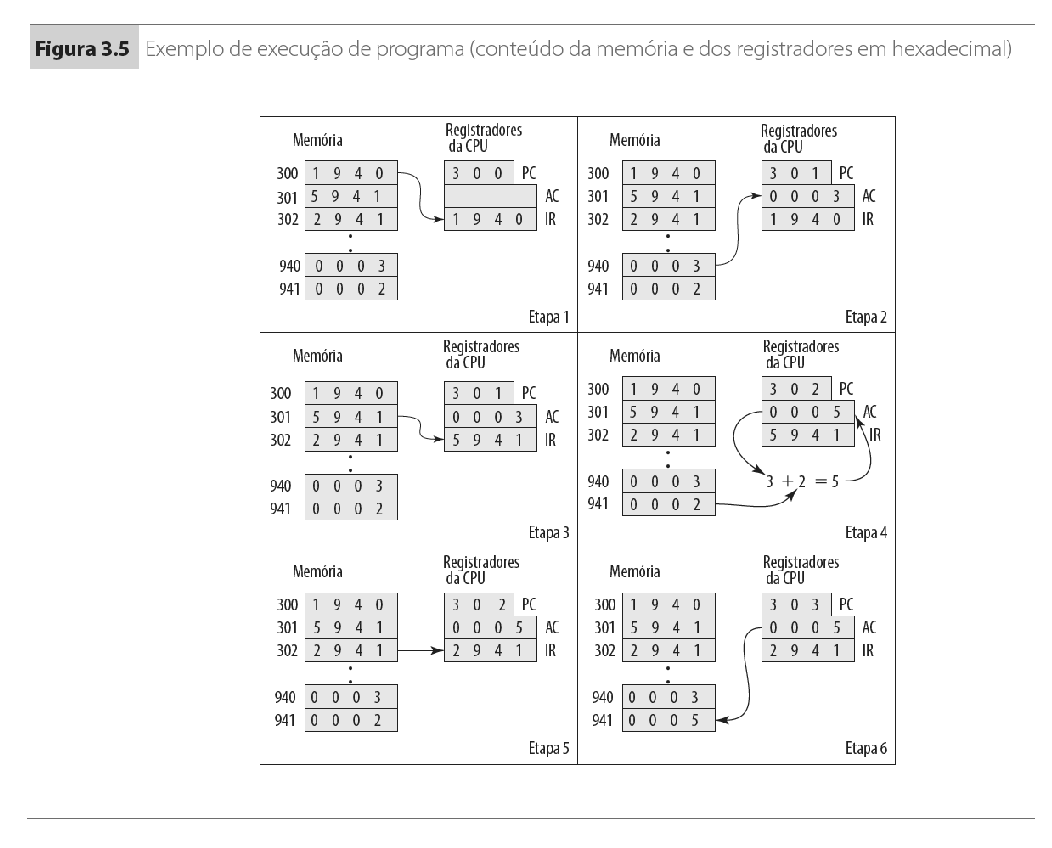
\includegraphics[height=0.8\textheight]{figs/exemplohpt.eps}
\end{slide}

\begin{slide}{Diagrama de estado}
   \centering
   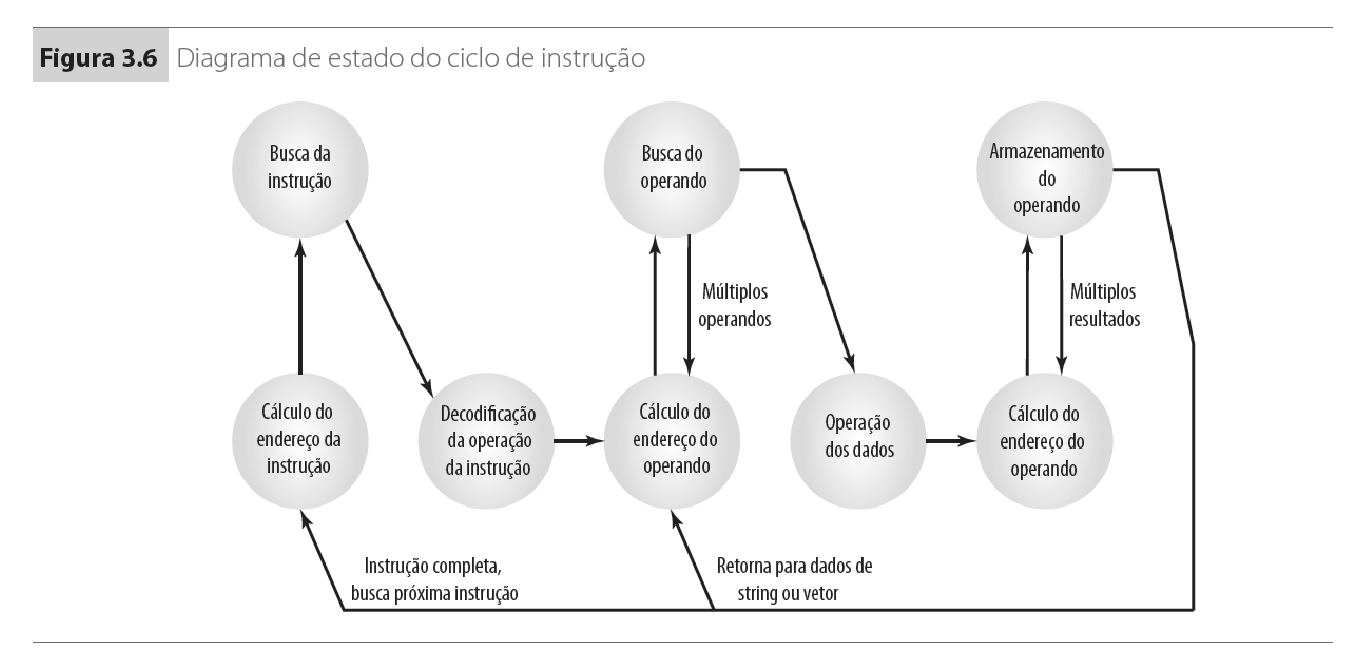
\includegraphics[width=\textwidth]{figs/instrestado.eps}
\end{slide}

%\section[slide=false]{Função do computador}
\begin{slide}{Interrupções}
\begin{itemize}
   \item Interrupção: alteração do processamento normal por elementos externos ao programa em execução 
   \item Classes:
   \begin{itemize}
      \item Programa (?)
      \item Timer
      \item E/S
      \item Falha de hardware
   \end{itemize}
   \item Objetivo: melhorar a eficiência do processamento.
\end{itemize}
\end{slide}

\begin{slide}{Fluxo de controle}
   \centering
   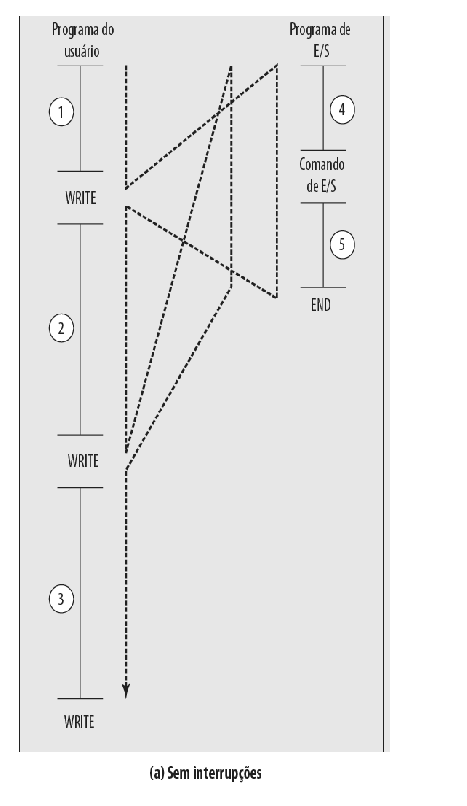
\includegraphics[height=0.8\textheight]{figs/int01.eps}
   \pause
   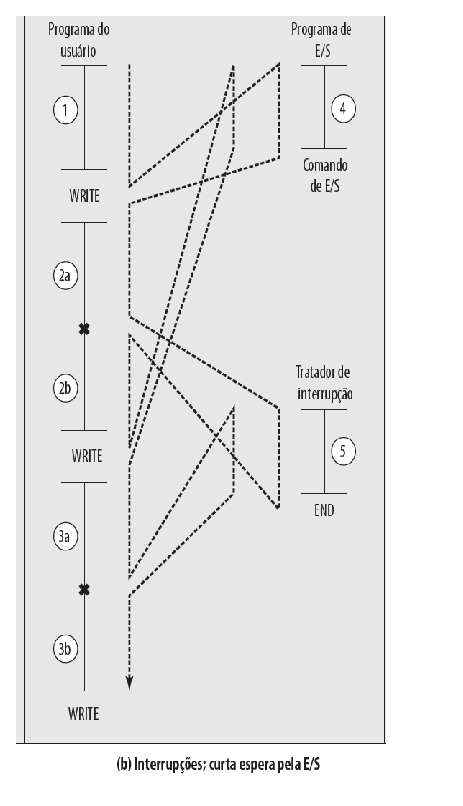
\includegraphics[height=0.8\textheight]{figs/int02.eps}
   \pause
   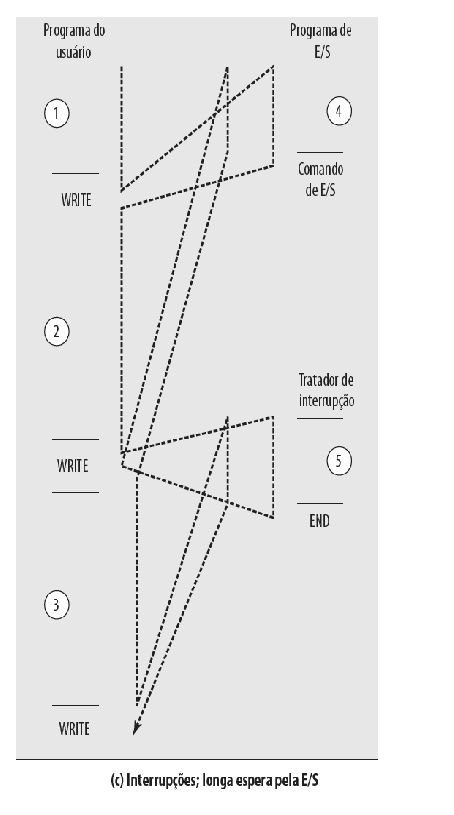
\includegraphics[height=0.8\textheight]{figs/int03.eps}
\end{slide}

\begin{slide}{Transferência de controle}
   \centering
   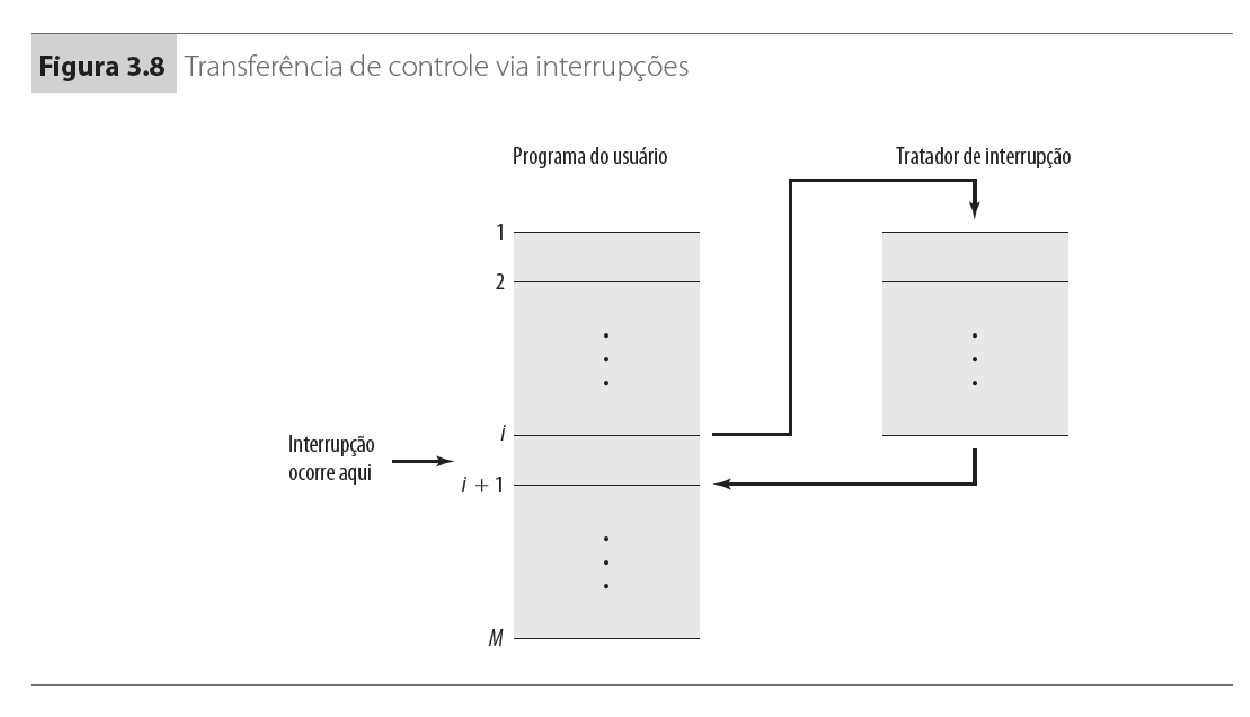
\includegraphics[height=0.75\textheight]{figs/int_transf.eps}
\end{slide}

\begin{slide}{Novo ciclo de instrução}
   \centering
   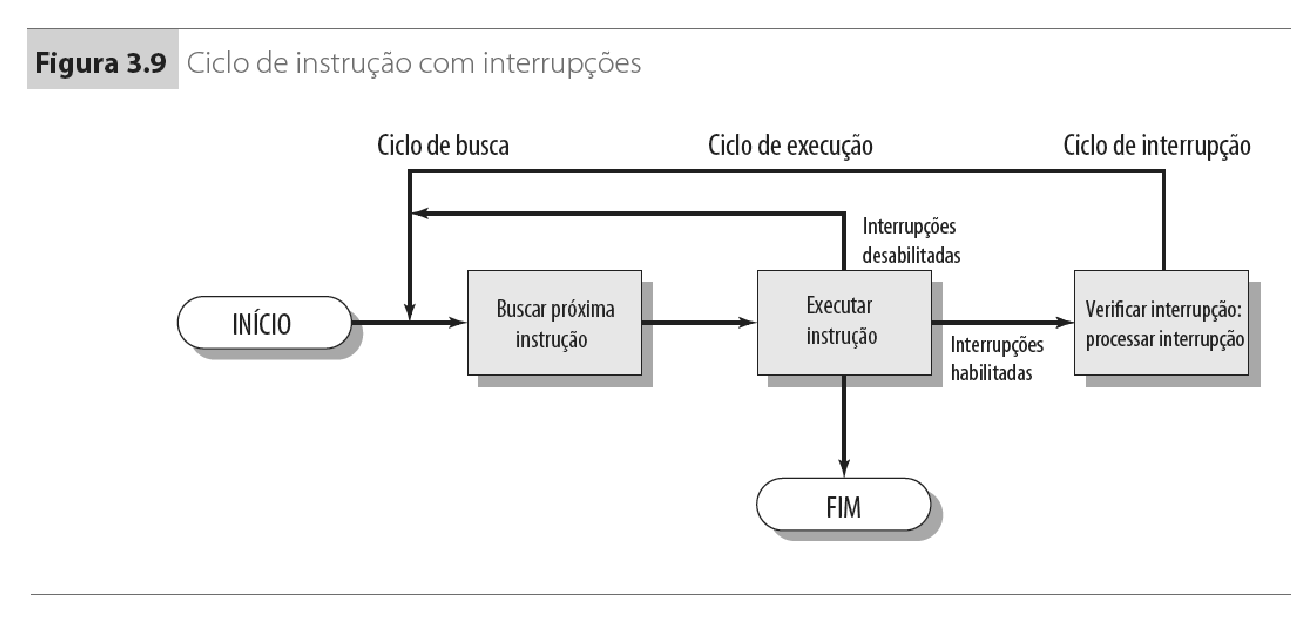
\includegraphics[width=\textwidth]{figs/int_ciclo.eps}
\end{slide}

\begin{slide}{Sincronização 1}
   \centering
   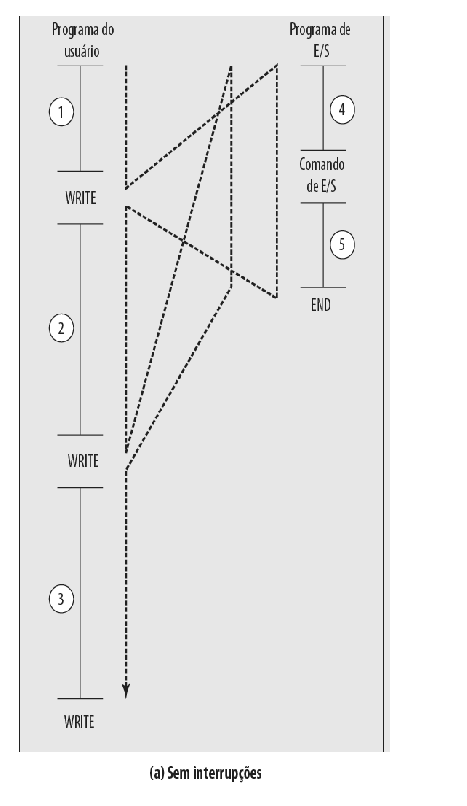
\includegraphics[height=0.8\textheight]{figs/int01.eps}
   \includegraphics[height=0.8\textheight]{figs/sinc1.eps}
\end{slide}

\begin{slide}{Sincronização 2}
   \centering
   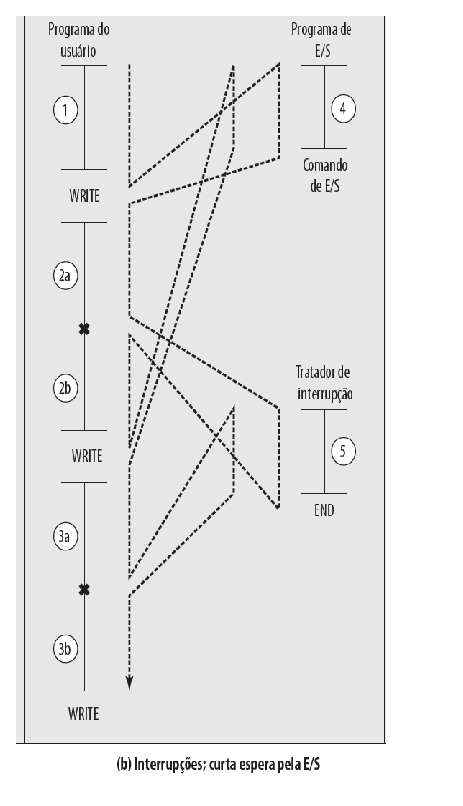
\includegraphics[height=0.8\textheight]{figs/int02.eps}
   \includegraphics[height=0.8\textheight]{figs/sinc1.eps}
\end{slide}

\begin{slide}{Sincronização 3}
   \centering
   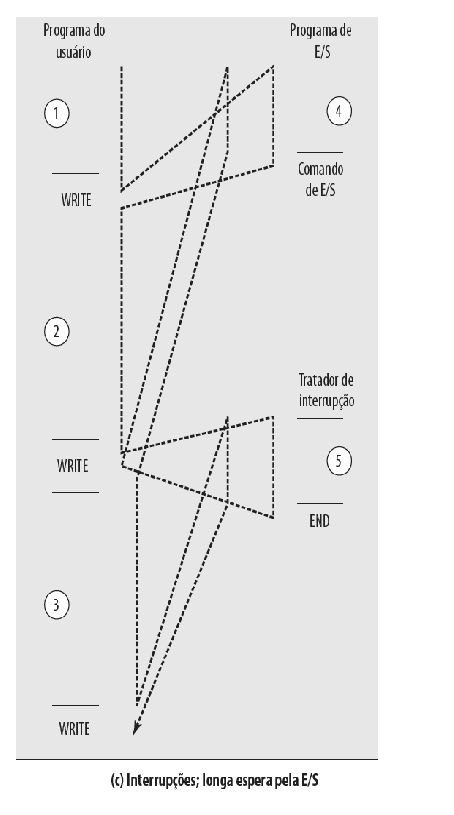
\includegraphics[height=0.8\textheight]{figs/int03.eps}
   \includegraphics[height=0.8\textheight]{figs/sinc2.eps}
\end{slide}

\begin{slide}{Diagrama de estado}
   \centering
   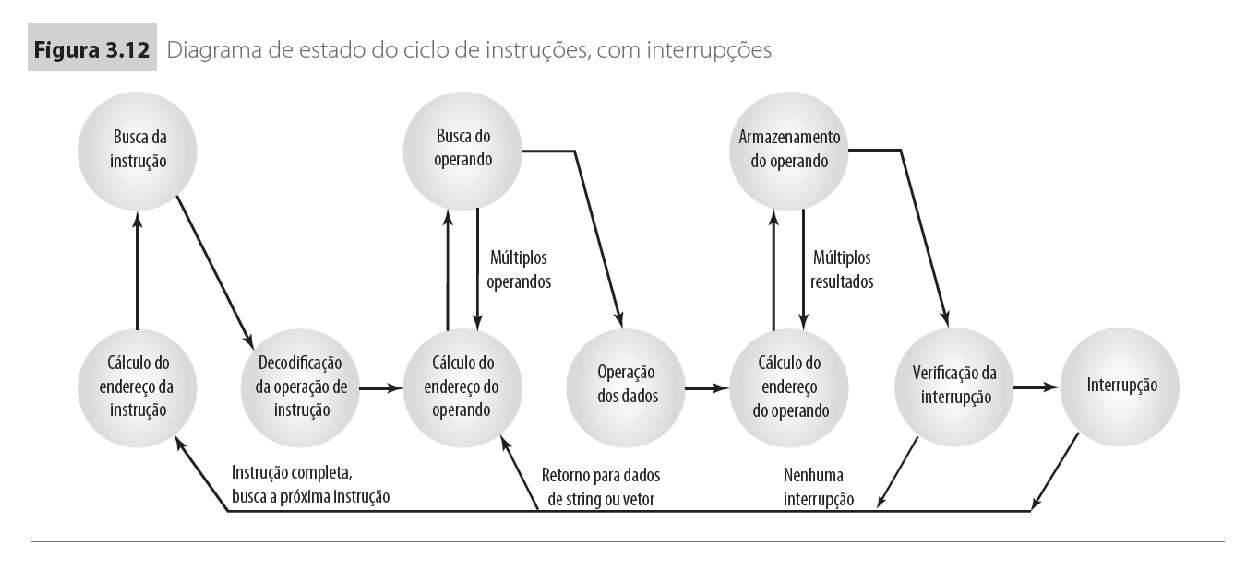
\includegraphics[width=\textwidth]{figs/int_estado.eps}
\end{slide}

\begin{slide}{Interrupções múltiplas}
\begin{itemize}
   \item Como proceder quando várias interrupções ocorrem durante o tratamento de uma outra interrupção?
   \item Abordagens:
   \begin{itemize}
      \item Processamento sequencial
      \item Processamento aninhado
      \item Processamento por prioridade
   \end{itemize}
\end{itemize}
\end{slide}

\begin{slide}{Sequencial e aninhado}
   \centering
   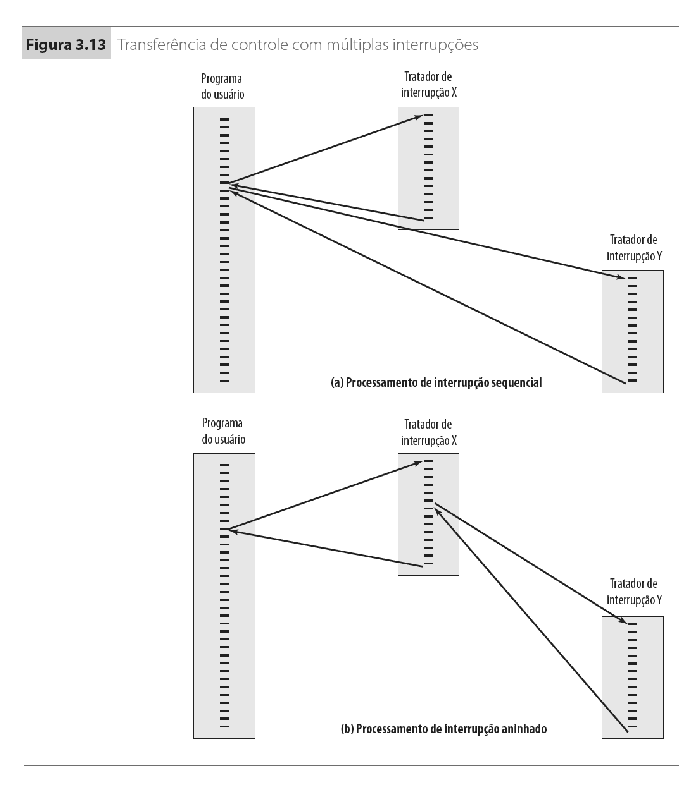
\includegraphics[height=0.8\textheight]{figs/multi1.eps}
\end{slide}

\begin{slide}{Por prioridade}
   \centering
   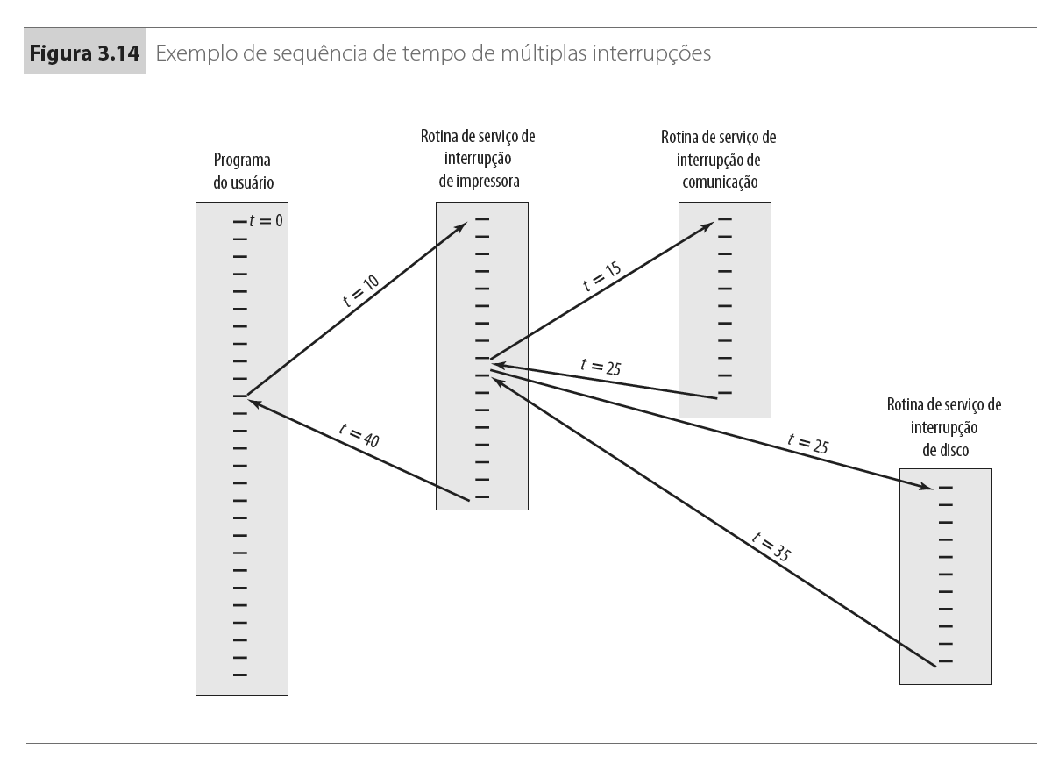
\includegraphics[height=0.8\textheight]{figs/multi2.eps}
\end{slide}
\end{document}
